\section{Differential Cross-Section}
\label{sec:differential cross-section}

The analysis method is very similar to the previously published one \cite{totem-8tev-1km}. The only important difference stems from using different RPs for the measurement: unit 210-fr instead of 220-nr as in \cite{totem-8tev-1km} since the latter was not equipped with sensors anymore. Due to the optics and beam parameters the unit 210-fr has worse low-$|t|$ acceptance, further deteriorated by the tilt of the unit (effectively increasing the RP distance from the beam). Consequently, in order to maintain the low-$|t|$ reach essential for this study, the main analysis (denoted ``2RP'') only uses the 220-fr units (thus 2 RPs per diagonal). Since not using the 210-nr units may, in principle, result in worse resolution and background suppression, for control reasons, the traditional analysis with 4 units per diagonal (denoted ``4RP'') was pursued, too. In Section~\ref{sec:cross checks} the ``2RP'' and ``4RP'' will be compared showing a very good agreement. In what follows, the ``2RP'' analysis will be described unless stated otherwise.

Section~\ref{sec:event analysis} covers all aspects related to the reconstruction of a single event. Section~\ref{sec:diff cs} describes the steps of transforming a raw $t$-distribution into the differential cross-section. The $t$-distributions are analysed separately for each LHC fill and each diagonal, and are only merged at the end as detailed in Section~\ref{sec:data merging}. Section~\ref{sec:systematics} describes the evaluation of systematic uncertainties and Section~\ref{sec:cross checks} presents several comparison plots used as systematic cross checks.

%----------------------------------------------------------------------------------------------------
\subsection{Event Analysis}
\label{sec:event analysis}

The event kinematics are determined from the coordinates of track hits in the RPs after proper alignment (see Sec.~\ref{sec:alignment}) using the LHC optics (see Sec.~\ref{sec:optics}).

%------------------------------

\subsubsection{Kinematics Reconstruction}
\label{sec:kinematics}

For each event candidate the scattering angles of both protons (one per arm) are first estimated separately. In the ``2RP'' analysis, these formulae are used:
\begin{equation}
\label{eq:kin 1a}
	\theta^{*\rm L,R}_x = {x\over L_x}\ ,\quad \theta^{*\rm L,R}_y = {y\over L_y}
\end{equation}
where L and R refer to the left and right arm, respectively, and $x$ and $y$ stand for the proton position in the 220-fr unit. This one-arm reconstruction is used for tagging of elastic events, where the left and right arm protons are compared.

Once a proton pair has been selected, both arms are used to reconstruct the kinematics of the event
\begin{equation}
\label{eq:kin 2a}
		\theta_x^* = {1\over 2} \left( \theta^{*\rm L}_x + \theta^{*\rm R}_x \right)\ ,\qquad
		\theta_y^* = {1\over 2} \left( \theta^{*\rm L}_y + \theta^{*\rm R}_y \right)\ .
\end{equation}
Thanks to the left-right symmetry of the optics and elastic events, this combination leads to cancellation of the vertex terms (cf.~Eq.~(\ref{eq:prot trans})) and thus to improvement of the angular resolution (see Section \ref{sec:resolution}).

Finally, the scattering angle, $\theta^*$, and the four-momentum transfer squared, $t$, are calculated:

\begin{equation}
\label{eq:th t}
\theta^* = \sqrt{{\theta_x^*}^2 + {\theta_y^*}^2}\ ,\qquad t = - p^2 ({\theta_x^*}^2 + {\theta_y^*}^2)\ ,
\end{equation}
where $p$ denotes the beam momentum.

In the ``4RP'' analysis, the same reconstruction as in \cite{totem-8tev-1km} is used which allows for stronger elastic-selection cuts, see Section~\ref{sec:tagging}.



%------------------------------

\subsubsection{Alignment}
\label{sec:alignment}

TOTEM's usual three-stage procedure (Section 3.4 in~\cite{totem-ijmp}) for correcting the detector positions and rotation angles has been applied: a beam-based alignment prior to the run followed by two offline methods. The first method uses straight tracks to determine the relative position among the RPs by minimising track-hit residuals. The second method exploits the symmetries of elastic scattering to determine the positions of RPs with respect to the beam. This determination is repeated in 20-minute time intervals to check for possible beam movements.

The alignment uncertainties have been estimated as $25\un{\mu m}$ (horizontal shift), $100\un{\mu m}$ (vertical shift) and $2\un{m rad}$ (rotation about the beam axis). They are larger than in some previous TOTEM publications (e.g.~Ref.~\cite{totem-jinst}) due to the lower instantaneous luminosity with $\beta^* = 2.5\un{km}$ and thus smaller statistics in every alignment time interval. Propagating the uncertainties through Eq.~(\ref{eq:kin 2a}) to reconstructed scattering angles yields $0.50\un{\mu rad}$ ($0.35\un{\mu rad}$) for the horizontal (vertical) angle. RP rotations induce a bias in the reconstructed scattering angles:
\begin{equation}
\label{eq:alig rot bias}
	\theta_x^* \rightarrow \theta_x^* + c \theta_y^*\ ,\quad
	\theta_y^* \rightarrow \theta_y^* + d \theta_x^*\ ,
\end{equation}
where the proportionality constants $c$ and $d$ have zero mean and standard deviations of $0.013$ and $0.00039$, respectively.



%------------------------------

\subsubsection{Optics}
\label{sec:optics}

It is crucial to know with high precision the LHC beam optics between IP5 and the RPs, i.e. the behaviour of the spectrometer composed of the various magnetic elements. The optics calibration has been applied as described in~\cite{totem-optics}. This method uses RP observables to determine fine corrections to the optical functions presented in Eq.~(\ref{eq:prot trans}).

In each arm, the residual errors induce a bias in the reconstructed scattering angles:
\begin{equation}
\label{eq:opt bias}
	\theta_x^* \rightarrow (1 + b_x)\, \theta_x^*\ ,\qquad
	\theta_y^* \rightarrow (1 + b_y)\, \theta_y^*\ ,
\end{equation}
where the biases $b_x$ and $b_y$ have uncertainties of $0.17\un{\%}$ and $0.15\un{\%}$, respectively, and a correlation factor of $-0.90$. To evaluate the impact on the $t$-distribution, it is convenient to decompose the correlated biases $b_x$ and $b_y$ into eigenvectors of the covariance matrix:
\begin{equation}
\label{eq:opt bias modes}
	\begin{aligned}
		\begin{pmatrix} b_x^{\rm L}\cr b_y^{\rm L} \cr b_x^{\rm R}\cr b_y^{\rm R} \end{pmatrix} =\ &
			\eta_1 \underbrace{\begin{pmatrix} -1.608\times10^{-3}\cr +1.473\times10^{-3}\cr -1.630\times10^{-3}\cr +1.477\times10^{-3} \end{pmatrix}}_{\rm mode\ 1}
  			\ +\ \eta_2 \underbrace{\begin{pmatrix} -5.157\times10^{-4}\cr +2.541\times10^{-5}\cr +5.566\times10^{-4}\cr +2.746\times10^{-5} \end{pmatrix}}_{\rm mode\ 2} \cr
  		&+\ \eta_3 \underbrace{\begin{pmatrix} +3.617\times10^{-4}\cr +3.625\times10^{-4}\cr +3.006\times10^{-4}\cr +3.641\times10^{-4} \end{pmatrix}}_{\rm mode\ 3}\ ,\cr
	\end{aligned}
\end{equation}
where the factors $\eta_{1,2,3}$ have zero mean and unit variance. The fourth eigenmode has a negligible contribution and therefore is not explicitly listed.



%------------------------------

\subsubsection{Resolution}
\label{sec:resolution}

\begin{figure}
\begin{center}
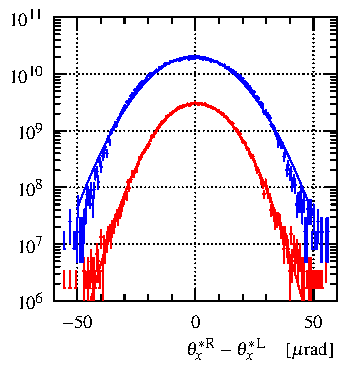
\includegraphics{fig/resolution_non_gaussianity.pdf}
\caption{%
Difference between horizontal scattering angles reconstructed in the right and left arm, for the diagonal 45 bottom - 56 top. Red: data from the beginning of fill 5317, blue: data from the fill end (vertically scaled $5\times$). The solid lines represent Gaussian fits.
}
\label{fig:resol x 1a}
\end{center}
\end{figure}

Two kinds of resolution can be distinguished: the resolution of the single-arm angular reconstruction, Eq.~(\ref{eq:kin 1a}), used for selection cuts and near-edge acceptance correction, and the resolution of the double-arm reconstruction, Eq.~(\ref{eq:kin 2a}), used for the unsmearing correction of the final $t$-distribution. Since the single-arm reconstruction is biased by the vertex term in the horizontal plane, the corresponding resolution is significantly worse than the double-arm reconstruction.

The single-arm resolution can be studied by comparing the angles reconstructed from the left and right arm, see an example in Figure~\ref{fig:resol x 1a}. The width of the distributions was found to grow slightly during the fills, compatible with the effect of beam emittance growth. The typical range was from $10.0$ to $14.5\un{\mu rad}$ for the horizontal projection and from $0.36$ to $0.38\un{\mu rad}$ for the vertical. The associated uncertainties were $0.3$ and $0.007$, respectively. As illustrated in Figure~\ref{fig:resol x 1a}, the shape of the distributions is very close to Gaussian, especially at the beginning of each fill.

Since in the vertical plane the resolution is driven by the beam divergence, the double-arm resolution can simply be scaled from the single-arm value: $\sigma(\theta^*_y) = (0.185 \pm 0.010)\un{\mu rad}$ where the uncertainty accounts for the full variation in time. In the horizontal plane the estimation is more complex due to several contributing smearing mechanisms. Therefore, a MC study was performed with two extreme sets of beam divergence, vertex size and sensor resolution values. These parameters were tuned within the ``4RP'' analysis where they are accessible thanks to the additional information from the 210-fr units. The study yielded $\sigma(\theta^*_x) =  (0.29 \pm 0.04)\un{\mu rad}$ where the uncertainty accounts for the full time variation.


%----------------------------------------------------------------------------------------------------
\subsection{Differential Cross-Section Reconstruction}
\label{sec:diff cs}

For a given $t$ bin, the differential cross-section is evaluated by selecting and counting elastic events:
\begin{equation}
{\d\sigma\over \d t}(\hbox{bin}) =
	\mathcal{N}\, \mathcal{U}(t)\, \mathcal{B}(t)\, {1\over \Delta t}
	\sum\limits_{\vbox{\scriptsize\hbox{\hskip0.7mm events}\vskip-1mm\hbox{$t\, \in\, {\rm bin}$}}} \mathcal{A}(\theta^*_x, \theta_y^*)\ \mathcal{E}(\theta_y^*)
	\ ,
\end{equation}
where $\Delta t$ is the width of the bin, $\mathcal{N}$ is a normalisation factor and the other symbols stand for various correction factors: $\mathcal{U}$ for unfolding of resolution effects, $\mathcal{B}$ for background subtraction, $\mathcal{A}$ for acceptance correction and $\mathcal{E}$ for detection and reconstruction efficiency.



%-------------------------

\subsubsection{Event Tagging}
\label{sec:tagging}


\begin{table}
\caption{The elastic selection cuts. The superscripts R and L refer to the right and left arm. The rightmost column gives a typical standard deviation of the cut distribution.
}
\label{tab:cuts}
\begin{center}
%\vskip-3mm
\begin{tabular}{ccc}\hline
number & cut & std.~dev.~($\equiv 1\sigma$)\cr\hline
\vrule width0pt height11pt
1 & $\theta_x^{*\rm R} - \theta_x^{*\rm L}$				& $14\un{\mu rad}$	\cr
2 & $\theta_y^{*\rm R} - \theta_y^{*\rm L}$				& $0.38\un{\mu rad}$	\cr\hline
\end{tabular}
\end{center}
\end{table}

Within the ``2RP'' analysis one may apply the cuts requiring the reconstructed-track collinearity between the left and the right arm, see Table~\ref{tab:cuts}. The correlation plots corresponding to these cuts are shown in Figure~\ref{fig:cuts}. 

In order to limit the selection inefficiency, the thresholds for the cuts are set to $4\un{\sigma}$. Applying the cuts at the $5\un{\sigma}$-level would yield about $0.1\un{\%}$ more events almost uniformly in every $|t|$-bin. This kind of inefficiency only contributes to a global scale factor, which is irrelevant for this analysis because the normalisation is taken from a different data set (cf. Section~\ref{sec:normalisation}).

In the ``4RP'' analysis, thanks to the additional information from the 210-fr units, more cuts can be applied (cf.~Table~2 in~\cite{totem-7tev-el}). In particular the left-right comparison of the reconstructed horizontal vertex position, $x^*$, and the vertical position-angle correlation in each arm. Furthermore, since the single-arm reconstruction can disentangle the contributions from $x^*$ and $\theta^*_x$, the angular resolution is better compared with the ``2RP'' analysis and consequently cut 1 in the ``4RP'' analysis is more efficient against background.

% * cut 1 is not very powerful to suppers protons with non-zero xi
% th_x_R - th_x_L = D_x / L_x * (xi_R + xi_L)
% cut condition: |th_x_R - th_x_L| < 4sigma ~ 56 urad
% that means that the cut is effective for |xi_R + xi_L| > L_x * T / D_x = 51m * 56 urad / 3cm ~ 0.09


\begin{figure}
\begin{center}
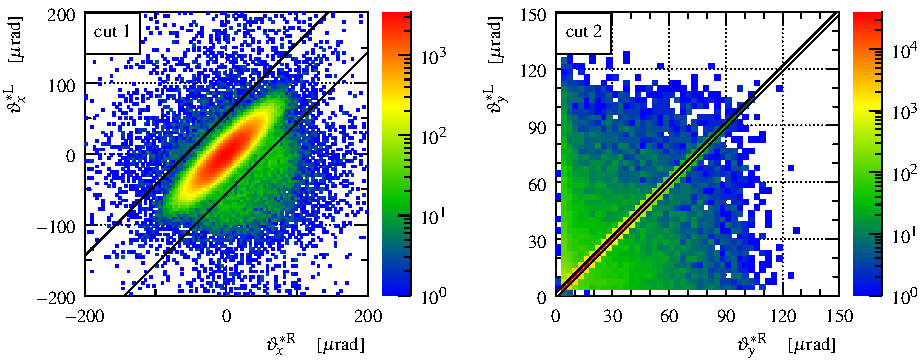
\includegraphics{fig/cut_example.pdf}
\caption{%
Correlation plots for the elastic event selection cuts presented in Table~\ref{tab:cuts} (``2RP'' analysis), showing events from the LHC fill 5313 and with diagonal topology 45 bottom -- 56 top. The solid black lines delimit the signal region within $\pm 4\un{\sigma}$.
}
\label{fig:cuts}
\end{center}
\end{figure}


%-------------------------

\subsubsection{Background}
\label{sec:background}

As the RPs were very close to the beam, one may expect an enhanced background from coincidence of beam halo protons hitting detectors in the two arms. Other background sources (pertinent to any elastic analysis) are central diffraction and pile-up of two single diffraction events.

The background rate (i.e.~impurity of the elastic tagging) is estimated in two steps, both based on distributions of discriminators from Table~\ref{tab:cuts} plotted in various situations, see an example in Figure~\ref{fig:tag bckg integ}. In the first step, diagonal data are studied under several cut combinations. While the central part (signal) remains essentially constant, the tails (background) are suppressed when the number of cuts is increased. In the second step, the background distribution is interpolated from the tails into the signal region. The form of the interpolation is inferred from non-diagonal RP track configurations (\textit{45 bottom -- 56 bottom} or \textit{45 top -- 56 top}), artificially treated like diagonal signatures by inverting the $y$ coordinate sign in the arm 45. These non-diagonal configurations cannot contain any elastic signal and hence consist purely of background which is expected to be similar in the diagonal and non-diagonal configurations. This expectation is supported by the agreement of the tails of the red, blue and green curves in the figure. Since the non-diagonal distributions are flat, the comparison of the signal-peak size to the amount of interpolated background yields an order-of-magnitue estimate of $1 - \mathcal{B} = \mathcal{O}(10^{-3})$.

\begin{figure}
\begin{center}
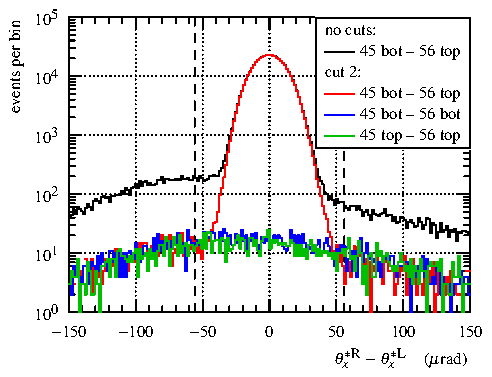
\includegraphics{fig/cut_dist_antidgn_cmp.pdf}
\caption{%
Distributions of discriminator 1, i.e. the difference between the horizontal scattering angle reconstructed from the right and the left arm. Data from LHC fill 5314. Black and red curves: data from diagonal 45 bottom -- 56 top, the different colours correspond to various combinations of the selection cuts (see numbering in Table~\ref{tab:cuts}). Blue and green curves: data from anti-diagonal RP configurations, obtained by inverting track $y$ coordinate in the left arm. The vertical dashed lines represent the boundaries of the signal region ($\pm 4\un{\sigma}$).
}
\label{fig:tag bckg integ}
\end{center}
\end{figure}

The $t$-distribution of the background can also be estimated by comparing data from diagonal and anti-diagonal configurations, as illustrated in Figure~\ref{fig:tag bckg dist}. The ratio background / (signal + background) can be obtained by dividing the blue or green histograms by the red or magenta histograms. Consequently, the background correction factor, $\mathcal{B}$, is estimated to be $0.9975 \pm 0.0010$ at $|t| = 0.001\un{GeV^2}$, $0.9992 \pm 0.0003$ at $|t| = 0.05\un{GeV^2}$ and $0.998 \pm 0.001$ at $|t| = 0.2\un{GeV^2}$. The uncertainty comes from statistical fluctuations in the histograms and from considering different diagonals and anti-diagonals.

\begin{figure}
\begin{center}
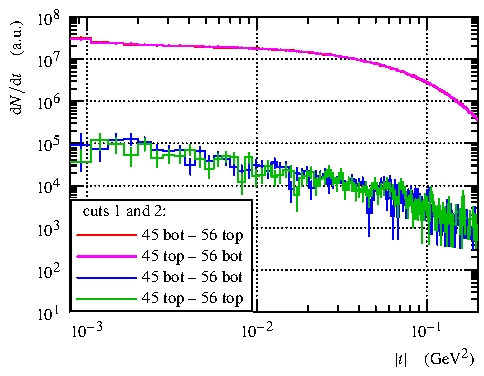
\includegraphics{fig/t_dist_antidgn_cmp.pdf}
\caption{%
Comparison of $|t|$-distributions from different diagonal (signal + background) and anti-diagonal (background) configurations, after all cuts and acceptance correction. Data from the LHC fill 5314.
}
\label{fig:tag bckg dist}
\end{center}
\end{figure}



%-------------------------

\subsubsection{Acceptance Correction}
\label{sec:acc corr}

The acceptance for elastic protons is limited mostly by two factors: sensor coverage (relevant for low $|\theta^*_y|$) and LHC beam aperture (at $|\theta^*_y| \approx 100\un{\mu rad}$). Since the 210-fr unit is tilted with respect to the 220-fr unit, the thin windows around sensors do not overlap perfectly. Therefore there are phase space regions where protons need to traverse thick walls of 210-fr RP before being detected in 220-fr RP. This induces reduced detection efficiency difficult to determine precisely. Consequently these regions (close to the sensor edge facing the beam) have been excluded from the fiducial region used in the analysis, see the magenta lines in Figure~\ref{fig:acc corr princ}.

\begin{figure}
\begin{center}
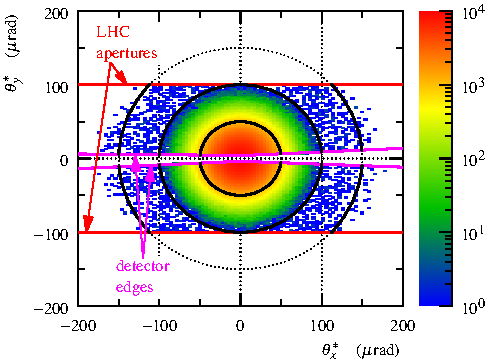
\includegraphics{fig/acc_phi_lab.pdf}
\caption{%
Distribution of scattering angle projections $\theta_y^*$ vs.~$\theta_x^*$, data from LHC fill 5317. The upper (lower) part comes from the diagonal 45 bottom -- 56 top (45 top -- 56 bottom). The red horizontal lines represent cuts due to the LHC apertures, the magenta lines cuts due to the RP edges. The dotted circles show contours of constant scattering angle $\theta^* = 50$, $100$ and $150\un{\mu rad}$. The parts of the contours within acceptance are emphasized in thick black.
}
\label{fig:acc corr princ}
\end{center}
\end{figure}

The correction for the above phase-space limitations includes two contributions -- a geometrical correction $\mathcal{A}_{\rm geom}$ reflecting the fraction of the phase space within the acceptance and a component $\mathcal{A}_{\rm fluct}$ correcting for fluctuations around the acceptance boundaries:
\begin{equation}
\mathcal{A}(\theta^*_x, \theta_y^*) = \mathcal{A}_{\rm geom}(\theta^*)\ \mathcal{A}_{\rm fluct}(\theta^*_x, \theta_y^*)\ .
\end{equation}

The calculation of the geometrical correction $\mathcal{A}_{\rm geom}$ is based on the azimuthal symmetry of elastic scattering, experimentally verified for the data within acceptance. As shown in Figure \ref{fig:acc corr princ}, for a given value of $\theta^*$ the correction is given by:
\begin{equation}
\label{eq:acc geom}
\mathcal{A_{\rm geom}}(\theta^*) = {
	\hbox{full circumference}\over 
	\hbox{arc length within acceptance}
} \ .
\end{equation}

The correction $\mathcal{A}_{\rm fluct}$ is calculated analytically from the probability that any of the two elastic protons leaves the region of acceptance due to the beam divergence. The beam divergence distribution is modelled as a Gaussian with the spread determined by the method described in Section~\ref{sec:resolution}. This contribution is sizeable only close to the acceptance limitations. Data from regions with corrections larger than $2$ are discarded.

The full acceptance correction, $\mathcal{A}$, has a value of $12$ in the lowest-$|t|$ bin and decreases smoothly towards about $2.1$ at $|t| = 0.2\un{GeV^2}$. Since a single diagonal cannot cover more than half of the phase space, the minimum value of the correction is $2$.

The uncertainties related to $\mathcal{A}_{\rm fluct}$ follow from the uncertainties of the resolution parameters: standard deviation and distribution shape, see Section~\ref{sec:resolution}. Since $\mathcal{A}_{\rm geom}$ is calculated from a trivial trigonometric formula, there is no uncertainty directly associated with it. However biases can arise indirectly from effects that break the assumed azimuthal symmetry like misalignments or optics perturbations already covered above.



%-------------------------

\subsubsection{Inefficiency Corrections}
\label{sec:ineff corr}

Since the overall normalisation will be determined from another dataset (see Section~\ref{sec:normalisation}), any inefficiency correction that does not alter the $t$-distribution shape does not need to be considered in this analysis (trigger, data acquisition and pile-up inefficiency discussed in~\cite{totem-7tev-el,totem-8tev-tot1}). The remaining inefficiencies are related to the inability of a RP to resolve the elastic proton track.

One such case is when a single RP does not detect and/or reconstruct a proton track, with no correlation to other RPs. This type of inefficiency, $\mathcal{I}_1$, is evaluated within the ``4RP'' analysis by removing the studied RP from the tagging cuts, repeating the event selection and calculating the fraction of recovered events. A typical example is given in Figure~\ref{fig:eff uncorr}, showing that the efficiency decreases gently with the vertical scattering angle. This dependence is reproduced with MC simulations and originates from the fact that protons with larger $|\theta_y^*|$ hit the RPs further from their edge and therefore the potentially created secondary particles have more chance to be detected. Since the RP detectors cannot resolve multiple tracks (non-unique association between ``U'' and ``V'' track candidates), the presence of a secondary particle track prevents from using the affected RP in the analysis. The $\mathcal{I}_1$ inefficiency includes several sources: nuclear scattering, delta rays, etc. As shown by the MC studies, only some of them give edge effects, that's why they are at about $0.5\un{\%}$ level.

\begin{figure}
\begin{center}
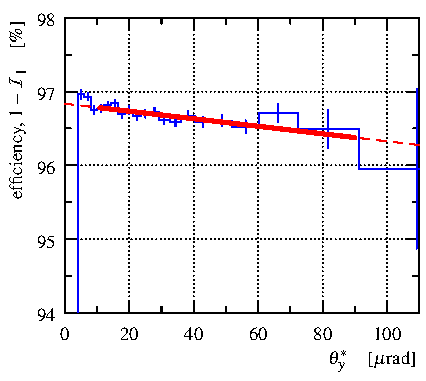
\includegraphics{fig/eff3outof4_fits.pdf}
\caption{%
Single-RP uncorrelated inefficiency for the 220-fr bottom RP in the right arm. The rapid drop at $\theta_y^* \approx 4\un{\mu rad}$ is due to acceptance effects at the sensor edge. The red lines represent a linear fit of the efficiency dependence on the vertical scattering angle (solid) and its extrapolation to the regions affected by acceptance effects (dashed).
}
\label{fig:eff uncorr}
\end{center}
\end{figure}

Proton interactions in a RP affecting simultaneously another RP downstream represent another source of inefficiency. The contribution from these correlated inefficiencies, $\mathcal{I}_2$, is determined by evaluating the rate of events with high track multiplicity ($\gtrsim$ 5) in both 210-fr and 220-fr RP units. Events with high track multiplicity simultaneously in the top and bottom RP of the 210-fr units are discarded as such a shower is likely to have started upstream from the RP station and thus be unrelated to the elastic proton interacting with detectors. The value, $\mathcal{I}_2 \approx (1.5 \pm 0.7)\un{\%}$, is compatible between left/right arms and top/bottom RP pairs and compares well to Monte-Carlo simulations (e.g.~section 7.5 in \cite{hubert-thesis}).

The full correction is calculated as
\begin{equation}
\label{efficiency}
	\mathcal{E}(\theta_y^*) = {1\over 1 - \left( \sum\limits_{i\in \rm RPs} \mathcal{I}^i_1(\theta_y^*) + 2 \mathcal{I}_2 \right) } \ .
\end{equation}
The first term in the parentheses sums the contributions from the diagonal RPs used in the analysis. In the ``2RP'' analysis it increases from about $6.9$ to $8.5\un{\%}$ from the lowest to the highest $|\theta_y^*|$, with an uncertainty of about $0.4\un{\%}$. For the ``4RP'' analysis, since more RPs contribute, the sum is greater: from $10.5$ to $13.0\un{\%}$ between the lowest to the highest $|\theta_y^*|$.



%-------------------------

\subsubsection{Unfolding of Resolution Effects}
\label{sec:unfolding}

Thanks to the very good resolution (see Section~\ref{sec:resolution}), the following iterative procedure can be safely used to evaluate the correction for resolution effects.
\begin{itemize}[noitemsep,topsep=0pt]
\item[1.] The differential cross-section data are fitted by a smooth curve.
\item[2.] The fit is used in a numerical-integration calculation of the smeared $t$-distribution (using the resolution parameters determined in Section~\ref{sec:resolution}). The ratio between the smeared and the non-smeared $t$-distributions gives a set of per-bin correction factors.
\item[3.] The corrections are applied to the observed (yet uncorrected) differential cross-section yielding a better estimate of the true $t$-distribution.
\item[4.] The corrected differential cross-section is fed back to step 1.
\end{itemize}
As the estimate of the true $t$-distribution improves, the difference between the correction factors obtained in two successive iterations decreases. When the difference becomes negligible, the iteration stops. This is typically achieved after the second iteration. 

The final correction $\mathcal{U}$ is significantly different from $1$ only at very low $|t|$ (where a rapid cross-section growth occurs, see Figure~\ref{fig:unfolding}). The relative effect is never greater than $0.4\un{\%}$.

Several fit parametrisations were tested, however yielding negligible difference in the final correction $\mathcal{U}$ for $|t| \lesssim 0.3\un{GeV^2}$. Figure~\ref{fig:unfolding} shows the case for two of those.

For the uncertainty estimate, the uncertainties of the $\theta_x^*$ and $\theta_y^*$ resolutions (see Section~\ref{sec:resolution}) as well as fit-model dependence have been taken into account. Altogether, the uncertainty is smaller than $0.1\un{\%}$.

\begin{figure}
\begin{center}
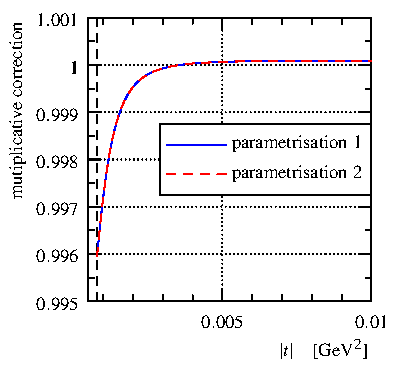
\includegraphics{fig/unfolding_num_int_model_cmp.pdf}
\caption{%
Unfolding correction as a function of $|t|$. The vertical dashed line indicates the position of the acceptance cut. The two correction curves were obtained with different fit parametrisations used in step 1 (see text).
}
\label{fig:unfolding}
\end{center}
\end{figure}



%-------------------------

\subsubsection{Normalisation}
\label{sec:normalisation}

The normalisation factor $\mathcal{N}$ is determined by requiring the integrated nuclear elastic cross-section to be $\sigma_{\rm el} = 31.0\un{mb}$ as obtained by TOTEM from a $\beta^* = 90\un{m}$ dataset at the same energy \cite{totem-13tev-90m}. The elastic cross-section is extracted from the data in two parts. The first part sums the $\d\sigma/\d t$ histogram bins for $0.01 < |t| < 0.5\un{GeV^2}$. The second part corresponds to the integral over $0 < |t| < 0.01\un{GeV^2}$ of an exponential fitted to the data on the interval $0.01 < |t| < 0.05\un{GeV^2}$.

The uncertainty of $\mathcal{N}$ is dominated by the $5.5\un{\%}$ uncertainty of $\sigma_{\rm el}$ from Ref.~\cite{totem-13tev-90m}.



%-------------------------

\subsubsection{Binning}
\label{sec:binning}

The bin sizes are set according to the $t$ resolution. Three different binnings are considered in this analysis: ``dense'' where the bin size is as large as the standard deviation of $|t|$, ``medium'' with bins twice as large and ``coarse'' with bins three times larger than the standard deviation of $|t|$.



%----------------------------------------------------------------------------------------------------

\subsection{Data Merging}
\label{sec:data merging}

After analysing the data in each diagonal and LHC fill separately, the individual differential cross-section distributions are merged. This is accomplished by a per-bin weighted average, with the weight given by inverse squared statistical uncertainty. The final cross-section values are listed in Table~\ref{tab:data} and are visualised in Figure~\ref{fig:dsdt}. The figure clearly shows a rapid cross-section rise below $|t| \lesssim 0.002\un{GeV^2}$ which, as interpreted later, is an effect due to the electromagnetic interaction.



%----------------------------------------------------------------------------------------------------

\subsection{Systematic Uncertainties}
\label{sec:systematics}

\begin{figure*}
\vskip-5mm
\begin{center}
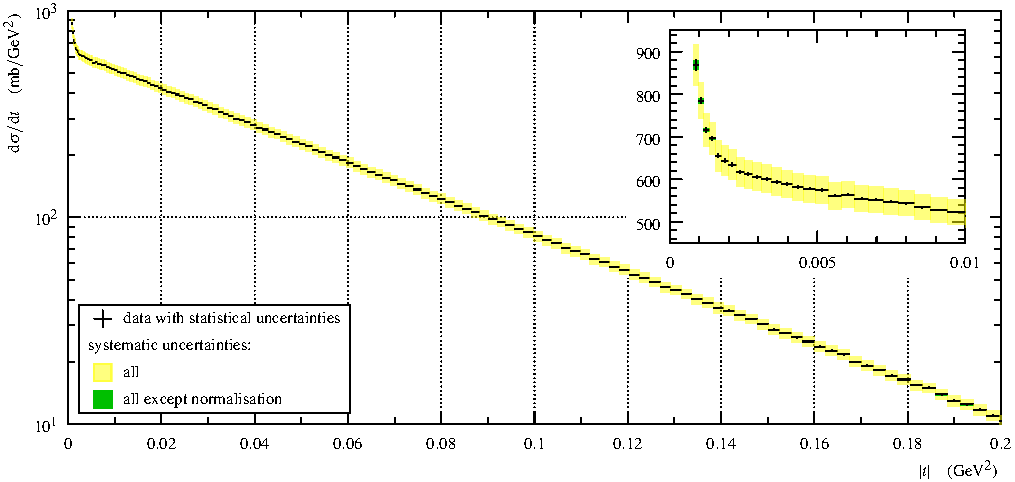
\includegraphics{fig/t_dist_tabulated.pdf}
\caption{%
Differential cross-section from Table \ref{tab:data} with statistical (bars) and systematic uncertainties (bands). The yellow band represents all systematic uncertainties, the green one all but normalisation. The bands are centred around the bin content. {\bf Inset}: a low-$|t|$ zoom of cross-section rise due to the Coulomb interaction.
}
\label{fig:dsdt}
\end{center}
\vskip-5mm
\end{figure*}


The following sources of systematic uncertainties have been considered.
\begin{itemize}[noitemsep,topsep=0pt]

\item Alignment: shifts in $\theta^*_{x,y}$ (see Section~\ref{sec:alignment}). Both left-right symmetric and anti-symmetric modes have been considered. In the vertical plane, both contributions correlated and uncorrelated between the diagonals have been considered.

\item Alignment $x$-$y$ tilts and optics: mixing between $\theta^*_{x}$ and $\theta^*_{y}$ (see Section~\ref{sec:alignment}). Both left-right symmetric and anti-symmetric modes have been considered.

\item Optics uncertainties: scaling of $\theta^*_{x,y}$ (see Section~\ref{sec:optics}). The three relevant modes in Eq.~(\ref{eq:opt bias}) have been considered.

\item Background subtraction (see Section~\ref{sec:background}): the $t$-dependent uncertainty of the correction factor $\mathcal{B}$.

\item Acceptance correction (see Section~\ref{sec:acc corr}): the uncertainty of resolution parameters, non-gaussianity of the resolution distributions, left-right asymmetry of the beam divergence.

\item Inefficiency corrections (see Section~\ref{sec:ineff corr}): for the uncorrelated inefficiency $\mathcal{I}_1$ both uncertainties of the fitted slope and intercept have been considered. For the correlated inefficiency $\mathcal{I}_2$ the uncertainty of its value has been considered.

\item The beam-momentum uncertainty: considered when the scattering angles are translated to $t$, see Eq.~(\ref{eq:th t}). The uncertainty was estimated by LHC experts as $0.1\un{\%}$ \cite{beam-mom-unc} in agreement with a previous assessment by TOTEM (Section~5.2.8.~in \cite{totem-8tev-90m}).

\item Unsmearing (see Section~\ref{sec:unfolding}): uncertainty of resolution parameters and model dependence of the fit.

\item Normalisation (see Section~\ref{sec:normalisation}): overall multiplicative factor.

\end{itemize}

For each error source, its effect on the $|t|$-distribution is evaluated with a Monte-Carlo simulation. It uses a fit of the final differential cross-section data to generate the true $t$-distribution and, in parallel, builds another $t$-distribution where the systematic error at $1\un{\sigma}$ level is introduced. The difference between the two $t$-distributions gives the systematic effect on the differential cross-section. This procedure is formally equivalent to evaluating
\begin{equation}
\label{eq:syst mode}
\delta s_{q}(t) \equiv \frac{\partial(\d\sigma/\d t)}{\partial q}\ \delta q\ ,
\end{equation}
where $\delta q$ corresponds to a $1\un{\sigma}$ bias in the quantity $q$ responsible for a given systematic effect.

The systematic uncertainty corresponding to the final differential cross-section merged from all the analysed LHC fills and both diagonals is propagated according to the same method as applied to the data, see Section~\ref{sec:data merging}. To be conservative, the systematic errors are assumed fully correlated among the four analysed LHC fills. The correlations between the two diagonals are respected for each systematic effect. This is particularly important for the vertical (mis)-alignment, as already noted in Ref.~\cite{totem-8tev-1km}. The relative position between the top and bottom RPs is known precisely from track-based alignment (see Sec.~\ref{sec:alignment}) and the leading component of residual misalignment is thus between the beam and a RP. Furthermore, whenever the beam were closer to a top RP, it would be further away from the corresponding bottom RP and vice versa. Consequently, the effect of the misalignment is predominantly anti-correlated between the diagonals. While the misalignment uncertainty in the lowest $|t|$ bin reaches about $7\un{\%}$ for a single diagonal, once the diagonals are merged the impact drops to about $1.2\un{\%}$.




\begin{figure*}
\begin{center}
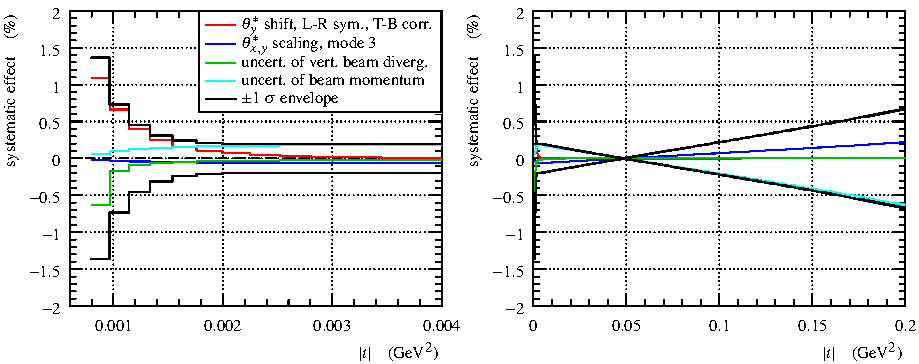
\includegraphics{fig/systematics_dgn_combination_summary.pdf}
\caption{%
Relative variation of the final differential cross-section due to systematic uncertainties (medium binning). The colourful histograms represent the leading uncertainties, each of them corresponds to a $1\un{\sigma}$ bias, cf.~Eq.~(\ref{eq:syst mode}). The envelope is determined by summing all considered contributions (except normalisation) in quadrature for each $|t|$ value.
}
\label{fig:syst unc}
\end{center}
\vskip-4mm
\end{figure*}



\begin{figure*}
%\vskip-3mm
\begin{center}
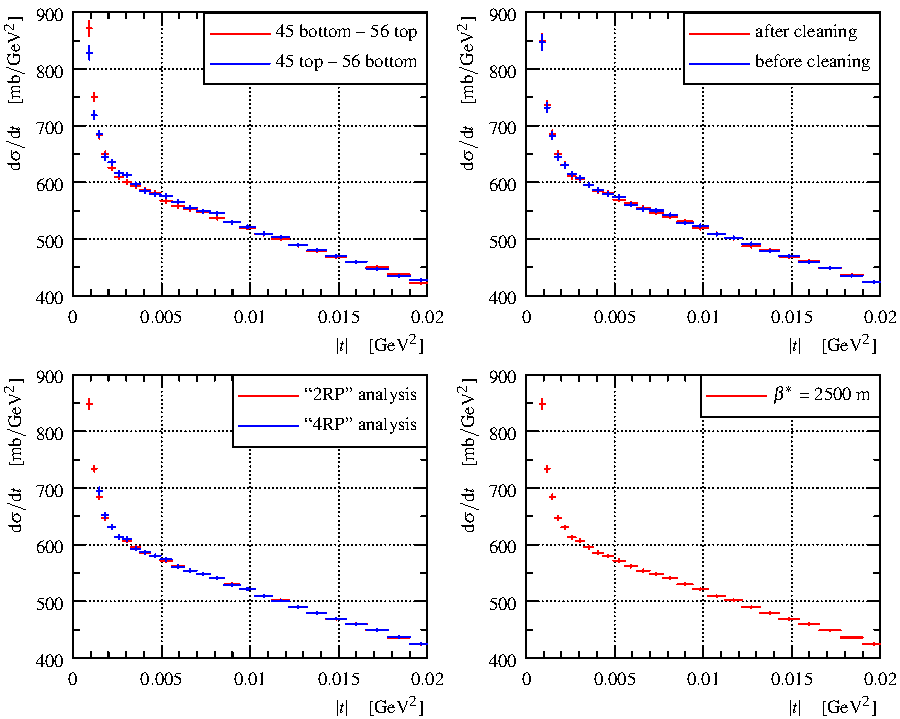
\includegraphics{fig/t_dist_cross_checks.pdf}
\caption{%
Collection of cross-check plots (medium binning, only statistical uncertainties are plotted).
{\bf Top left}: comparison of results from the two diagonals, data from all LHC fills.
{\bf Top right}: comparison of results from time periods after and before beam cleanings, data from all LHC fills and both diagonals.
{\bf Bottom left}: comparison of results from ``2RP'' and ``4RP'' analyses, data from all LHC fills and both diagonals.
{\bf Bottom right}: comparison of results obtained from two different data-takings at the same energy but with different optics. The blue histogram is taken from Ref.~\cite{totem-13tev-90m}.
}
\label{fig:dsdt checks}
\end{center}
\end{figure*}



The leading uncertainties (except normalisation) are shown in Figure~\ref{fig:syst unc}. At low $|t|$ they include the vertical alignment (left-right symmetric, top-bottom correlated) and the uncertainty of the vertical beam divergence. At higher $|t|$ values, the uncertainties are dominated by the beam momentum and optics uncertainties (mode 3 in Eq.~(\ref{eq:opt bias modes})). These leading effects are listed in Table~\ref{tab:data} which can be used to approximate the covariance matrix of systematic uncertainties:
\begin{equation}
\label{eq:covar mat}
\mat V_{ij} = \sum_{q} \delta s_{q}(i)\ \delta s_{q}(j)\: ,
\end{equation}
where $i$ and $j$ are bin indices (row numbers in Table~\ref{tab:data}) and the sum goes over the leading error contributions $q$ (five rightmost columns in the table).


%----------------------------------------------------------------------------------------------------

\subsection{Systematic Cross-Checks}
\label{sec:cross checks}

Compatible results have been obtained by analysing data subsets of events from different bunches, different diagonals (Figure~\ref{fig:dsdt checks}, top left), different fills and different time periods -- in particular those right after and right before the beam cleanings (Figure~\ref{fig:dsdt checks}, top right). Figure~\ref{fig:dsdt checks}, bottom left, shows that both analysis approaches, ``2RP'' and ``4RP'', yield compatible results. The relatively large difference between the diagonals at very low $|t|$ (Figure~\ref{fig:dsdt checks}, top left) is fully within the uncertainty due to the vertical misalignment, see Section~\ref{sec:systematics}.

Figure~\ref{fig:dsdt checks}, bottom right, shows an excellent agreement between the data from this analysis and previous results obtained with $\beta^* = 90\un{m}$ optics \cite{totem-13tev-90m}.


%----------------------------------------------------------------------------------------------------



\input data_table.tex
